%
% File acl2020.tex
%
%% Based on the style files for ACL 2020, which were
%% Based on the style files for ACL 2018, NAACL 2018/19, which were
%% Based on the style files for ACL-2015, with some improvements
%%  taken from the NAACL-2016 style
%% Based on the style files for ACL-2014, which were, in turn,
%% based on ACL-2013, ACL-2012, ACL-2011, ACL-2010, ACL-IJCNLP-2009,
%% EACL-2009, IJCNLP-2008...
%% Based on the style files for EACL 2006 by 
%%e.agirre@ehu.es or Sergi.Balari@uab.es
%% and that of ACL 08 by Joakim Nivre and Noah Smith

\documentclass[11pt,a4paper]{article}
\usepackage[hyperref]{acl2020}
\usepackage{booktabs}
\usepackage{graphicx}
\usepackage{times}
\usepackage{latexsym}
\renewcommand{\UrlFont}{\ttfamily\small}

\usepackage{microtype}

\aclfinalcopy % Uncomment this line for the final submission


\newcommand\BibTeX{B\textsc{ib}\TeX}

\title{Netflix Movie Recomendation System}

\author{Gavin Galusha \\
  Tulane University \\
  \texttt{email@domain} \\\And
  Bob Seger \\
  Night Moves U / Detroit, MI \\
  \texttt{email@domain} \\}

\date{}

\begin{document}
\maketitle
\begin{abstract}
Lorem ipsum dolor sit amet, consectetur adipiscing elit, sed do eiusmod tempor incididunt ut labore et dolore magna aliqua. Ut enim ad minim veniam, quis nostrud exercitation ullamco laboris nisi ut aliquip ex ea commodo consequat. Duis aute irure dolor in reprehenderit in voluptate velit esse cillum dolore eu fugiat nulla pariatur. Excepteur sint occaecat cupidatat non proident, sunt in culpa qui officia deserunt mollit anim id est laborum.
\end{abstract}


\section{Introduction}

For our Project, we are building a Movie recomendation system. The project is built on an ensemble of methods: Firstly, Collaborative-Filtering filtering is a way to reccomend movies to a user, based off the preferences of that user. In this case, this would be the movies this specific user has rated.
By aggregating the feature vector of each item (movie) a user has reviewed, we can build this user profile. From here we can use cosine similarity to compute the similarity between users. This already gives us a great start in predicting which movies a user may like, because odds are it is one that someone else
who shares their movie taste also likes.

While user - user similarity is important, we also want to calculate the similarity of movie - movie. To build profiles for these movies that we will later compare, we must perform a variety of NLP techniques in order to obtain the various features of each movie. This mainly
comes in the form of generating embeddings for the movie descriptions, as well as the mood, genre, and tag of the film. Capturing these features on a semantic level is important for comparison, and is relevant because films with genres like "thriller" and "horror" will now be considered similar. Simple categorical encoding fails to catch these dimensions.




Lorem ipsum dolor sit amet, consectetur adipiscing elit, sed do eiusmod tempor incididunt ut labore et dolore magna aliqua. Ut enim ad minim veniam, quis nostrud exercitation ullamco laboris nisi ut aliquip ex ea commodo consequat. Duis aute irure dolor in reprehenderit in voluptate velit esse cillum dolore eu fugiat nulla pariatur. Excepteur sint occaecat cupidatat non proident, sunt in culpa qui officia deserunt mollit anim id est laborum.

\section{Related Work}

Citations within the text appear in parentheses as~\citep{aho1972theory} or, if the author's name appears in the text itself, as \citet{andrew2007scalable}.



Lorem ipsum dolor sit amet, consectetur adipiscing elit, sed do eiusmod tempor incididunt ut labore et dolore magna aliqua. Ut enim ad minim veniam, quis nostrud exercitation ullamco laboris nisi ut aliquip ex ea commodo consequat. Duis aute irure dolor in reprehenderit in voluptate velit esse cillum dolore eu fugiat nulla pariatur. Excepteur sint occaecat cupidatat non proident, sunt in culpa qui officia deserunt mollit anim id est laborum.


\section{Methods}

Data Preparation:
There are two primary datasets that we have used for this project: https://www.kaggle.com/datasets/grouplens/movielens-20m-dataset/code and https://www.kaggle.com/datasets/ashpalsingh1525/netflixLinks. The first dataset contains a variety of dataframes all linked together with keys like userId, movieId, and tagId.
This one is essential for user-user collaborative filtering. The second dataset contains specific movie attributes, like description, duration, cast, etc. This one is ideal for calculating movie-movie similarity. The first step was to join together the various dataframes, and string together a cohesive data frame with 
no missing values.

Mood Prediction:
Our first step in the overall process of movie generation, was to try to guess the mood of a movie based off it's other features. For this, we started by using CountVectorizer to create embeddings for the description sentences. We used one-hot encoding for the categorical features, and paired these with the embeddings generated by the descriptions as the input to predict the mood class for each film.
Next, we performed our train-test-split, and fit a logistic regression model for classification. We 

Cosin Similarity:
In experiments2, we took our first crack at cosine similarity. For this task, we sought to find the cosine similarity between movies by first performing NLP techniques on the 


\section{Results}

Lorem ipsum dolor sit amet, consectetur adipiscing elit, sed do eiusmod tempor incididunt ut labore et dolore magna aliqua. Ut enim ad minim veniam, quis nostrud exercitation ullamco laboris nisi ut aliquip ex ea commodo consequat. Duis aute irure dolor in reprehenderit in voluptate velit esse cillum dolore eu fugiat nulla pariatur. Excepteur sint occaecat cupidatat non proident, sunt in culpa qui officia deserunt mollit anim id est laborum.


Table~\ref{tab:a_table} shows a table. Note that we refer to output generated by \texttt{Experiments.ipynb}. This way, whenever we re-run our notebook, we can regenerate the paper with the latest results.

\begin{table}[ht]
\centering
% note that we can refer to tables generated by our Experiments.ipynb notbook.
\begin{tabular}{rr}
\toprule
   C &   F1 \\
\midrule
 0.1 & 0.90 \\
 1.0 & 0.92 \\
 5.0 & 0.93 \\
10.0 & 0.89 \\
\bottomrule
\end{tabular}

\caption{\label{tab:a_table} A caption. }
\end{table}

Figure~\ref{fig:a_label} shows a figure

\begin{figure}[ht]
	\centering
	% note that we can refer to figures generated by our Experiments.ipynb notbook.
	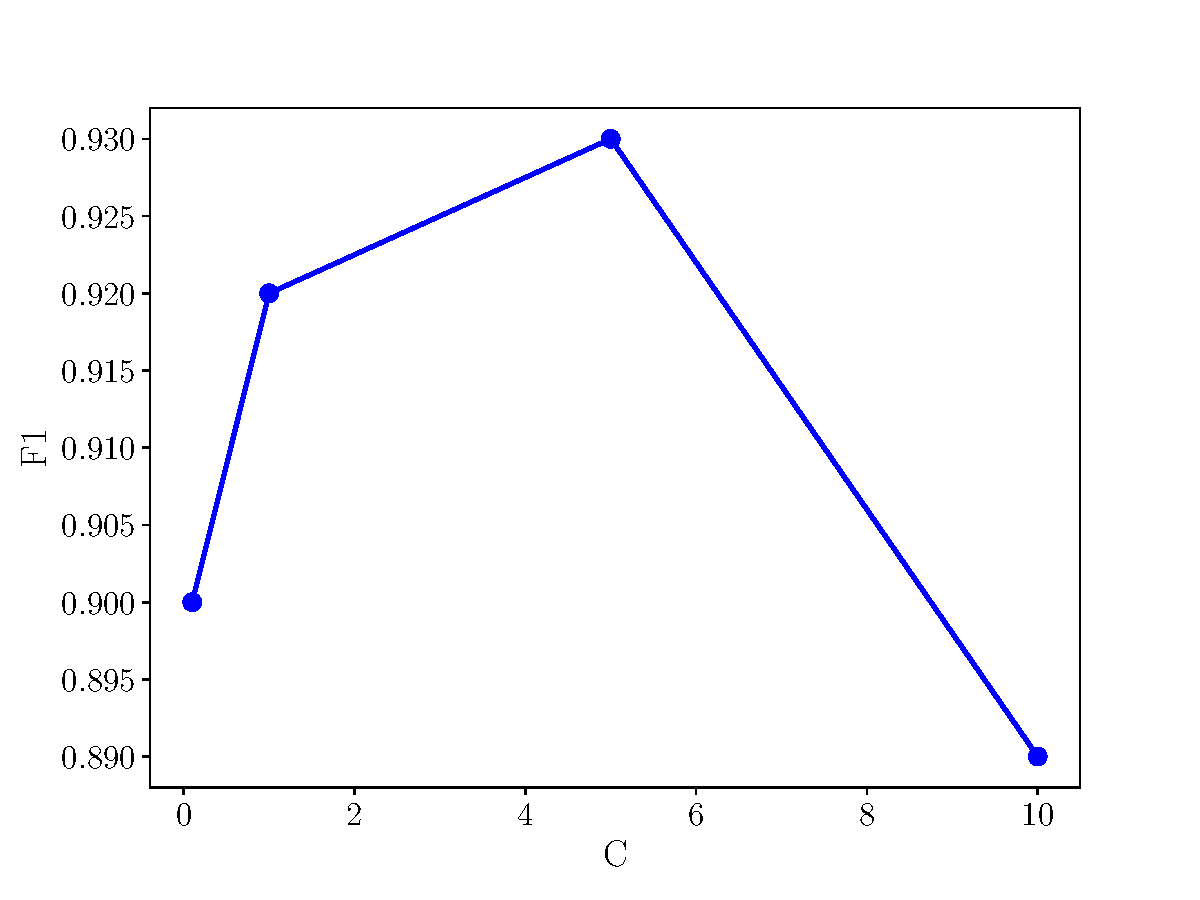
\includegraphics[width=3.5in]{../notebooks/results.pdf}
	\caption{A caption}
	\label{fig:a_label}
\end{figure}

\section{Discussion}

Lorem ipsum dolor sit amet, consectetur adipiscing elit, sed do eiusmod tempor incididunt ut labore et dolore magna aliqua. Ut enim ad minim veniam, quis nostrud exercitation ullamco laboris nisi ut aliquip ex ea commodo consequat. Duis aute irure dolor in reprehenderit in voluptate velit esse cillum dolore eu fugiat nulla pariatur. Excepteur sint occaecat cupidatat non proident, sunt in culpa qui officia deserunt mollit anim id est laborum.


\section{Conclusion}
Lorem ipsum dolor sit amet, consectetur adipiscing elit, sed do eiusmod tempor incididunt ut labore et dolore magna aliqua. Ut enim ad minim veniam, quis nostrud exercitation ullamco laboris nisi ut aliquip ex ea commodo consequat. Duis aute irure dolor in reprehenderit in voluptate velit esse cillum dolore eu fugiat nulla pariatur. Excepteur sint occaecat cupidatat non proident, sunt in culpa qui officia deserunt mollit anim id est laborum.


\section{Division of Labor}
Lorem ipsum dolor sit amet, consectetur adipiscing elit, sed do eiusmod tempor incididunt ut labore et dolore magna aliqua. Ut enim ad minim veniam, quis nostrud exercitation ullamco laboris nisi ut aliquip ex ea commodo consequat. Duis aute irure dolor in reprehenderit in voluptate velit esse cillum dolore eu fugiat nulla pariatur. Excepteur sint occaecat cupidatat non proident, sunt in culpa qui officia deserunt mollit anim id est laborum.





\bibliography{references}
\bibliographystyle{acl_natbib}


\end{document}
